\documentclass{beamer}
\usepackage{graphicx}

\usetheme{default}

\beamertemplatenavigationsymbolsempty

\title{Prueba de Oposición JTP}
\author{Eric Brandwein}
\date{\today}

\begin{document}

\begin{frame}
    \titlepage
\end{frame}

\begin{frame}{}
    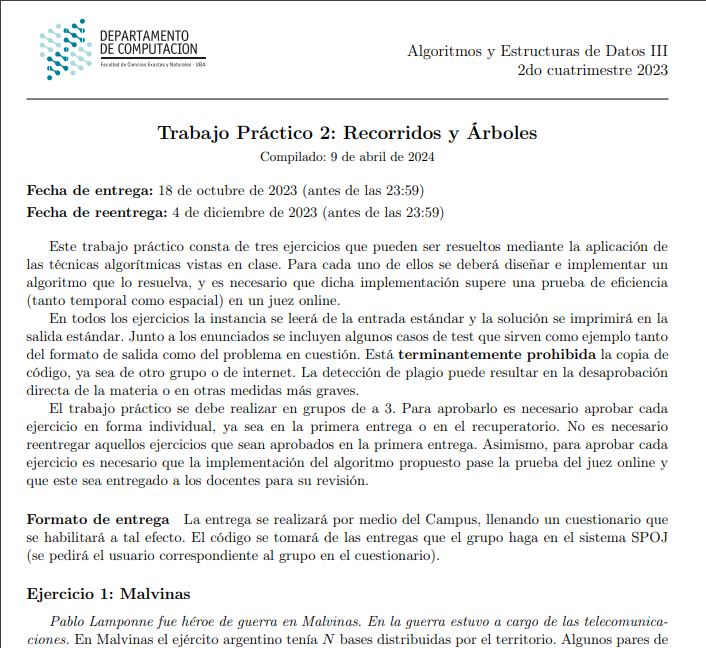
\includegraphics[trim={1mm 0 0 1mm}, clip, width=\textwidth]{img/titulo-tp.png}
\end{frame}

\begin{frame}{Contenidos previos}
    \begin{itemize}
        \item Estructuras de datos
        \item Complejidad temporal y espacial
        \item<2-> Técnicas algorítmicas
        \begin{itemize}
            \item Backtracking
            \item Programación dinámica
            \item Greedy
        \end{itemize}
    \end{itemize}
\end{frame}

\begin{frame}{Temario de este TP}
    \begin{itemize}
        \item Grafos y su representación
        \item Recorridos sobre grafos (BFS y DFS)
        \begin{itemize}
            \item Complejidad
            \item Propiedades de las estructuras resultantes
        \end{itemize}
        \item Árboles y sus propiedades
        \item Árboles generadores mínimos (AGM)
        \begin{itemize}
            \item Algoritmos para calcularlos (Prim, Kruskal)
            \item Propiedades de los AGM
        \end{itemize}
    \end{itemize}
\end{frame}


\begin{frame}{A verlo...}
\end{frame}


\begin{frame}
    \Huge \centering \structure{¡Muchas gracias!}
\end{frame}

\end{document}
